\documentclass{article}
\usepackage[utf8]{inputenc}
\usepackage{amsmath}
\usepackage{url}
\usepackage{amsfonts}
\usepackage{graphicx}
\usepackage{wrapfig}
\usepackage{xspace}
\usepackage{relsize}


\newcommand{\smartsolver}{\mbox{S\textsmaller[1]{3}}\xspace}
\newcommand{\SAT}{{SAT}}
\newcommand{\HLL}{{HLL}}
\newcommand{\LLL}{{LLL}}
\newcommand{\openETCS}{\textsf{openETCS}}
\newcommand{\ETCS}{\textsf{ETCS}}
\newcommand{\SCADE}{\textsc{Scade}}
\newcommand{\eg}{\textit{e.g.}}
\newcommand{\ie}{\textit{i.e.}}




\begin{document}
\title{Verification of \SCADE{} models with \smartsolver{} model-checker}
\author{Marielle Petit-Doche, Matthias Güdemann, Roméo Courbis\\Systerel}
\date{\today}

\maketitle

\begin{abstract}
This document describes the verification and validation processes applicable to \SCADE{} models using the \smartsolver{} model-checker.
\end{abstract}

\tableofcontents

\newpage

\section{Introduction}

This document gives a description of the VnV process applied on a \SCADE{} design model.
The \SCADE{} model covers two functions of the ETCS on-board unit:
\begin{description}
\item[Level Management function], described in SRS-26 §5.10
\item[Mode Management function], described in SRS-26, §4.6, §5.4, 5.6, 5.7, 5.9, 5.11, 5.13, 5.19
\end{description}

\section{Verification processes applicable to a\\SCADE{}~model}

The principe of verification consists in the definition of properties in textual languages, and verification of these properties by model-checking techniques on a textual translation of the \SCADE{} Model.


\begin{figure}[h!]
\centering
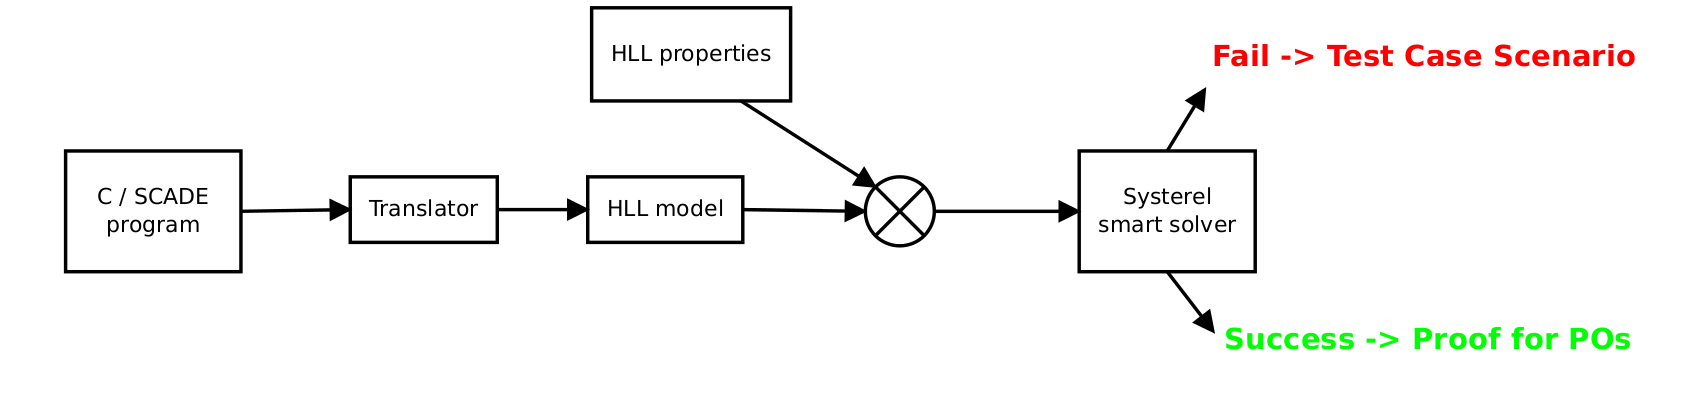
\includegraphics[width=1\textwidth]{S3_process}
\caption{Procedure of verification of \SCADE{} model}
\label{fig:procos}
\end{figure}

Figure \ref{fig:procos} describes the process:
\begin{itemize}
\item the main input is a \SCADE{} model to  verify (same approach and tool can be applied to a C program) which is translated in a High Level Language (a textual description of the model)
\item the second input is the properties to verify, written in \HLL{}
\item these both inputs are merged in a unique \HLL{} file, used directly as input of the Systerel Smart Solver (\smartsolver{} model-checker) for verification
\item result of the \smartsolver{} tool is Success or Failure; in case of failure counter-example is provided for analysis.
\end{itemize}

The \smartsolver{} tool is a model-checker which manages as well an internal \SAT{} solver as external \SAT{} solvers.

This process can be apply to cover three purposes:


\paragraph{ Properties of an \HLL{} Model: } The prover may be used to prove or disprove properties of an \HLL{} model. Those properties are modeled as proof obligations.
\begin{figure}[h!]
\centering
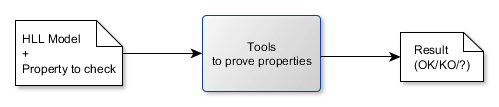
\includegraphics[width=1\textwidth]{Use_property_checker}
\caption{Properties of an \HLL{} Model}
\label{fig:proch}
\end{figure}

\paragraph{ Solving Properties of an \HLL{} Model: } The prover may be used as a solver, by finding values for the streams that comply with some property P. To do so, just put the negation of P as a proof obligation. If the prover succeeds to disprove the proof obligation, it will provide a solution solving P. If the prover succeeds to prove the proof obligation, then this proves that the property cannot be solved. This solution can be used to defined test cases too.
\begin{figure}[h!]
\centering
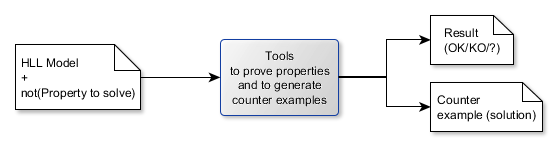
\includegraphics[width=1\textwidth]{Use_property_solver}
\caption{Solving Properties of an \HLL{} Model}
\label{fig:prosolv}
\end{figure}

\paragraph{ Proving the Equivalence of 2 \HLL{} Models: } The prover may be used to prove that 2 \HLL{} models with the same interface (the same input streams and output streams) are equivalent. To do so, an equivalent model is produced with proof obligations stating that for all input streams values, each output of the first \HLL{} model is equal to the output of the second model with the same name.
\begin{figure}[h!]
\centering
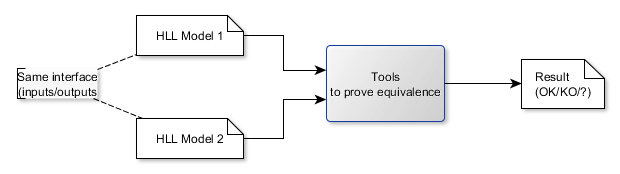
\includegraphics[width=1\textwidth]{Use_equivalence_checker}
\caption{Proving the Equivalence of 2 \HLL{} Models}
\label{fig:eqch}
\end{figure}


\section{Specified properties and results}

\begin{tabular}{|l|l|l|l|l}
\hline
\textbf{Name} & \textbf{Type} & \textbf{Model} & \textbf{SRS coverage} & \textbf{section} \\ \hline
isolate & simple proof & Modes  & 4.6.2 C1 &\\
no\_power & simple proof & Modes  & 4.6.2 C4 &\\
level case & use case & Level  & 5.10 &\\
shunting initiated by driver & validation & Modes  & 5.6 &\\
start of mission & validation & Modes  & 5.4 &\\
%\hline
%ManageModes & start\_of\_mission\_topnode.hll \\
\hline
\end{tabular}


\subsection{Application of \smartsolver{}: Static analysis}
\label{sec:static-analysis}

At first, the formal verification of the model was used to find bugs in the developed
\SCADE{} model.
\smartsolver{} adds some proof obligations to assess that the \HLL{}
model is correctly defined:
\begin{itemize}
\item Indexes of arrays belong to their ranges
\item Latch definition range check
\item No division by 0
\item No overflow and no underflow on arithmetic expressions
\item Output and constraint initialization check
\end{itemize}

Besides, the translators from a language to \HLL{} can also generate proof obligations to be analyzed by \smartsolver{},
to check that the code does not have undefined behavior with respect to the source language.

For example the C-translator adds some proof obligations to ensure conformance with the C99 standard.


\paragraph{Results}
The three models have been verified on their topnode:

\begin{tabular}{|l|l|l|}
\hline
\textbf{\SCADE{} model} & \textbf{Top Node} & \textbf{Results}  \\ \hline
Modes & ManageModes &  PO 1-5: valid \\
Levels & ManageLevels &  PO 1-5: valid \\
ModesAndLevels & ManageLevelAndMode & PO 1-5: valid \\
\hline
\end{tabular}

\subsubsection{Conditions to Isolate mode}
\label{sec:isolate}

\paragraph{Files used for the proof} The proof is defined in the file \url{https://github.com/openETCS/validation/blob/master/VnVUserStories/VnVUserStorySysterel/05-Work/S3/Small_Proof/isolate.hll} and it is verified on the top node \emph{ManageModes} of the \SCADE{} model \emph{Modes}.


\paragraph{What is proved ?}
The Condition 1 of SRS § 4.6 "The driver isolates the ERTMS/ETCS on-board equipment" is proved, ie; as soon as the input of \SCADE{} model \texttt{Data\_From\_DMI.'ETCS\_Isolated'} becomes true, the output \texttt{currentMode} becomes 'isolated' (\texttt{Level\_And\_Mode\_Types\_Pkg::IS}) and internal condition  is activated.


\paragraph{Constraints used}

None.

\paragraph{Results}

The property is proved.

\subsection{Verification of use case}

\emph{levels}


\paragraph{Files used for the proof} The proof is defined in the file \url{https://github.com/openETCS/validation/blob/master/VnVUserStories/VnVUserStorySysterel/05-Work/S3/Proof_SoM/shunting_initiated_by_driver.hll} and it is verified on the top node \emph{xxx} of the \SCADE{} model \emph{Level Management}.

\paragraph{What is proved ?}


\paragraph{Constraints used}


\paragraph{Results}


\subsection{Validation of informal specification}

\subsubsection{Procedure Shunting initiated by Driver}

\paragraph{Files used for the proof} The proof is defined in the file \url{https://github.com/openETCS/validation/blob/master/VnVUserStories/VnVUserStorySysterel/05-Work/S3/Proof_SoM/shunting_initiated_by_driver.hll} and it is verified on the node \emph{Procedure\_SH\_Initiated\_By\_Driver} of the \SCADE{} model \emph{Modes Management}. The same proof is also defined in the file \url{https://github.com/openETCS/validation/blob/master/VnVUserStories/VnVUserStorySysterel/05-Work/S3/Proof_SoM/shunting_initiated_by_driver_topnode.hll} to be verified on the top node \emph{ManageModes} of the \SCADE{} model \emph{Modes Management}.

\paragraph{What is proved ?}
We want to prove that the procedure SH\_Initiated\_By\_Driver is a
correct implementation of the section 5.6 Shunting Initiated By Driver of SRS-26.

To prove this, a specification of the flowchart is proposed in the
property file. However, the flowchart is not entirely specified:
elements \texttt{D030}, \texttt{A030}, \texttt{A095}, \texttt{S100} and
\texttt{A115} of the flow chart in SRS-26 are out of the scope of the mode management function.

\paragraph{Constraints used}
One hypothesis is used in this model to avoid a counter-example: when we are in \texttt{A100} the request of ``End of
Mission'' procedure correspond to the value of the input
\texttt{On-going Mission} as it is specified in the \SCADE{} model.

This hypothesis is justified by the fact that, according to
\texttt{A050}, \texttt{D040} and \texttt{A100}, if the input
\texttt{On-going Mission} is \texttt{True} then the ``End of Mission''
request is \texttt{True}, so equal to \texttt{On-going Mission}. Also,
as transition to SH mode is enable (\texttt{A050}) when ``End of
Mission'' request is made, the system should go to SH mode (or another
mode except SB mode). 

\paragraph{Results}
Considering the constraint and our model, the \SCADE{} model of
SH\_Initiated\_By\_Driver corresponds to the specification. Proof of this property allow to detect an error in \SCADE{} model: operator \emph{AND} was used instead operator \emph{OR}.
Besides the specification in \SCADE{}  of the computation of the output \emph{End\_Of\_Mission} was corrected.

\subsubsection{Procedure Start of Mission}

\paragraph{Files used for the proof}
The proof is defined in the file \url{https://github.com/openETCS/validation/blob/master/VnVUserStories/VnVUserStorySysterel/05-Work/S3/Proof_SoM/startofmission_topnode_proof.hll} and it is verified on the node \emph{Procedure\_StartOfMission} of the \SCADE{} model \emph{Modes}.


\paragraph{What is proved ?}
We want to prove that the procedure Procedure\_StartOfMission is a
correct implementation of the section 5.6 Procedure Start of mission of SRS-26.

Only the down part of the flowchart, from S10 and from S20, relative to the modes management, is specified in the \SCADE{} model.





\paragraph{Constraints used}
\begin{enumerate}
\item Level should not change : Level can be change at the beginning of Start of Mission procedure, but when we go in the step of mode selection, the level should not change.

\item Train Data should not change : Train Data are validated at the beginning of Start of Mission procedure, they shall be valid to start mode selection and we consider then that  their validity should not change.

\item The train shall stay at standstill during all the procedure. Indeed in Stand-By mode, standstill shall be ensure by supervision function (see SRS-26 §4.4.7.1.5).

\item The ``On Going Mission'' variable, input of SH Initiated by Driver, is
forced to False. This is justified by SRS 5, section ``5.4.6 Entry to
Mode Considered as a Mission''.
\end{enumerate}



\paragraph{Results}
Considering constraints and our \HLL{} model, the \SCADE{} model of Procedure
Start of Mission corresponds to the specification.
Some errors have been detected in the \SCADE{} model: links between nodes were wrong.

\subsubsection{Procedure On-Sight}
\emph{On going work}


\paragraph{Files used for the proof} The proof is defined in the file \url{https://github.com/openETCS/validation/blob/master/VnVUserStories/VnVUserStorySysterel/05-Work/S3/Proof_SoM/xxx} and it is verified on the top node \emph{xxx} of the \SCADE{} model \emph{Modes Management}.

\paragraph{What is proved ?}


\paragraph{Constraints used}


\paragraph{Results}


\subsection{Comparison of \SCADE{} models}

\emph{levels}\\
\\

\paragraph{Files used for the proof} The proof is defined in the file \url{https://github.com/openETCS/validation/blob/master/VnVUserStories/VnVUserStorySysterel/05-Work/S3/Proof_SoM/shunting_initiated_by_driver.hll} and it is verified on the top node \emph{xxx} of the \SCADE{} model \emph{Level Management}.

\paragraph{What is proved ?}


\paragraph{Constraints used}


\paragraph{Results}


\section{Conclusion}


\end{document}